% Slide 9 | Results | M3 (Tanishk Tasgaonkar) | 1:45 | E1: how accurately can kappa be estimated?
\begin{frame}{E1: estimating the speed $\kappa$ is biased}
\framesubtitle{Slide 9 \textbullet\ Results \textbullet\ M3 \textbullet\ 1:45}
\vspace{-2pt}
\begin{columns}[T,onlytextwidth]
\column{0.52\textwidth}
  \centering
  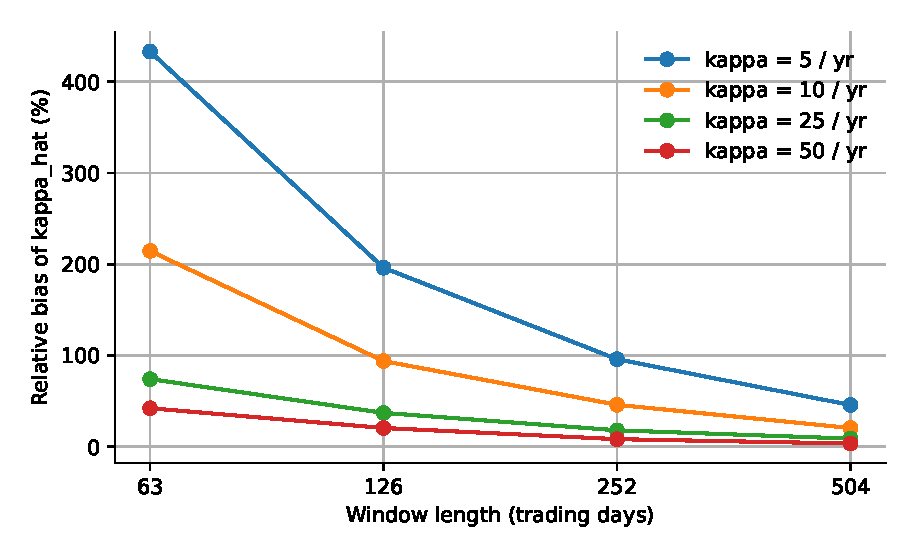
\includegraphics[width=\linewidth]{fig_e1_ou_estimation}
\column{0.44\textwidth}
  \footnotesize\raggedright
  \begin{itemize}\setlength{\itemsep}{3pt}
    \item one year of data: $\hat\kappa$ too high by \textbf{18\%} (7-day half-life) and \textbf{96\%} (35-day)
    \item the error halves each time the window doubles
  \end{itemize}
\end{columns}
\pairTakeaway{Pairs look faster, and more attractive, than they really are.}
\end{frame}
